\documentclass[../mainfile.tex]{subfile}
\author{Barbara Wiedermann}
\begin{document}
	\section{Folgen und Reihen}
	\subsection{Grundidee}
	 	Baggersee 1500m\textsuperscript{2} Fläche er wird so ausgehoben, dass er jede Woche um 200m\textsuperscript{2} wächst Algen breiten sich aus.\\
	 	Am Beginn: 1m\textsuperscript{2} -\textgreater Verdreifacht sich wöchentlich\\
	 	
\begin{tabular}{|l|l|l|l|l|l|l|}
\hline
(n)Wochen    & 0    & 1    & 2    & 3    & 4...    & 8    \\ \hline
See Fläche   & 1500 & 1700 & 1900 & 2500 & 2300... & 3100 \\ \hline
Algen Fläche & 1    & 3    & 9    & 27   & 81...   & 6561 \\ \hline
\end{tabular}\\\\\\
Gesetz: Seefläche: $1500+200n$\\
Algenfläche: $i*3^n$\\
$n \epsilon \mathbb{N}_0$ \\

\subsection{Definition}
Eine Folge ist eine Abbildung: \\
f: $\mathbb{N}$ -$>$ $\mathbb{R}$ bzw. f: $\mathbb{N}$ -$>$ $\mathbb{C}$\\
($\mathbb{N}$ manchmal)\\

\begin{figure}[!htbp]
\centering
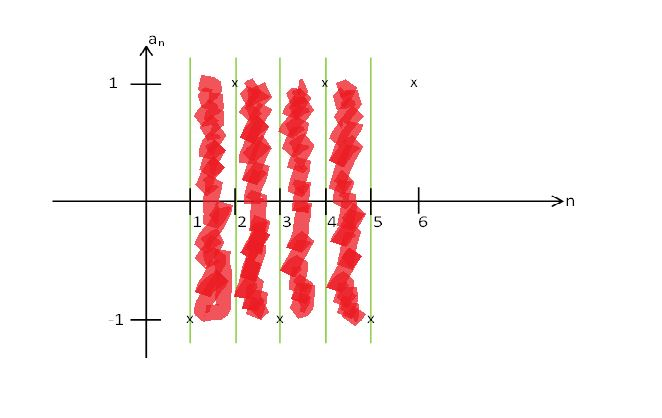
\includegraphics[width=10cm]{./bwiedermann/img/Zeichnung.jpg}
\caption{Darstellung einer Folge}
\end{figure}


\end{document}